% ============================================================
%  cap07.tex  --  Capítulo 7: Análise de Investimentos
%  Baseado em: Notas de Aula 6 + 8 (Cap. 6)
%  Referência: Bueno, Rangel & Santos, Cap. 6
% ============================================================

\chapter{Análise de Investimentos}

\section{Risco e Retorno: Introdução}

Todo investimento envolve um \textbf{trade-off} fundamental:
\begin{itemize}
  \item Projetos com mesmo retorno: escolher o de \textbf{menor risco}.
  \item Projetos com mesmo risco: escolher o de \textbf{maior retorno}.
\end{itemize}

Para mensurar e comparar projetos, três ferramentas centrais são:
\begin{enumerate}[label=\textbf{\arabic*.}]
  \item \textbf{VPL} (Valor Presente Líquido): maximiza o lucro absoluto.
  \item \textbf{TIR} (Taxa Interna de Retorno): mede a rentabilidade relativa.
  \item \textbf{TIRM} (TIR Modificada): corrige uma limitação da TIR.
\end{enumerate}

% ─────────────────────────────────────────────────────────────────────────────
\section{Valor Presente Líquido (VPL)}

\begin{definicao}
Dado um projeto com investimento inicial $P$ e fluxos de receita $\{R_1, R_2, \ldots, R_n\}$,
o \textbf{Valor Presente Líquido} é:
\[
  \VPL(i) = -P + \sum_{t=1}^n \frac{R_t}{(1+i)^t}
           = \sum_{t=1}^n \frac{R_t}{(1+i)^t} - P,
\]
onde $i$ é a \textbf{taxa livre de risco} (custo de oportunidade), usada para trazer
todas as despesas e receitas ao mesmo momento do tempo.
\end{definicao}

\subsection{Regra de decisão}

\begin{resultado}
\[
  \begin{cases}
  \VPL > 0: & \text{custo de oportunidade} < \TIR \quad\Rightarrow\quad \text{vale investir;} \\
  \VPL = 0: & \text{equilíbrio econômico}\quad (i = \TIR); \\
  \VPL < 0: & \text{custo de oportunidade} > \TIR \quad\Rightarrow\quad \text{não vale investir.}
  \end{cases}
\]
\end{resultado}

\subsection{Propriedades da função VPL}

Admitindo todos os fluxos intermediários positivos ($R_t > 0$), a função $\VPL(i)$ é:
\begin{itemize}
  \item \textbf{Decrescente}: $\VPL'(i) < 0$ (maior desconto $\Rightarrow$ menor VP das receitas);
  \item \textbf{Convexa}: $\VPL''(i) > 0$.
\end{itemize}

\begin{center}
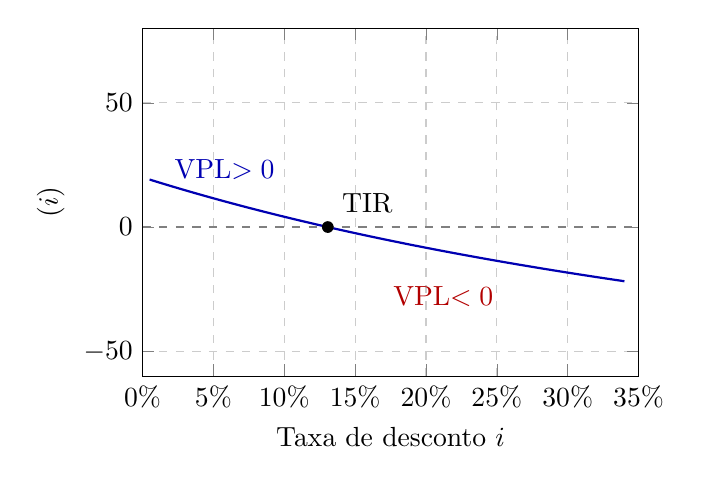
\begin{tikzpicture}
\begin{axis}[
  width=0.65\textwidth, height=6cm,
  xlabel={Taxa de desconto $i$},
  ylabel={$\VPL(i)$},
  xmin=0, xmax=0.35,
  ymin=-60, ymax=80,
  grid=major, grid style={dashed, gray!40},
  xtick={0,0.05,...,0.35},
  xticklabel={\pgfmathparse{\tick*100}\pgfmathprintnumber{\pgfmathresult}\%},
  legend pos=north east, legend style={font=\small},
]
  \addplot[thick, color=blue!70!black, domain=0.005:0.34, samples=60]
    {60/(1+x) + 60/(1+x)^2 - 100};
  \addplot[dashed, gray] coordinates {(0,0)(0.35,0)};
  \node[circle, fill=black, inner sep=1.5pt, label={above right:$\mathrm{TIR}$}]
        at (axis cs:0.1307,0) {};
  \node[above left, color=blue!70!black] at (axis cs:0.1,15) {VPL$>0$};
  \node[below right, color=red!70!black] at (axis cs:0.17,-20) {VPL$<0$};
\end{axis}
\end{tikzpicture}
\end{center}

% ─────────────────────────────────────────────────────────────────────────────
\section{Taxa Interna de Retorno (TIR)}

\begin{definicao}
A \textbf{TIR} é a taxa $r^*$ que zera o VPL:
\[
  P = \sum_{t=1}^n \frac{R_t}{(1+r^*)^t}
  \quad\Leftrightarrow\quad
  \VPL(r^*) = 0.
\]
\end{definicao}

\begin{exemplo}{TIR simples}
Investimento de R\$\,100 que retorna R\$\,60 ao final do 1º e do 2º ano:
\[
  100 = \frac{60}{1+r} + \frac{60}{(1+r)^2}
  \quad\Rightarrow\quad r \approx 13{,}07\%.
\]
Se a taxa livre de risco for $10\%$, vale investir.
\end{exemplo}

\subsection{Unicidade da TIR -- Regra de Descartes}

A equação $\VPL(r) = 0$ é um polinômio de grau $n$ em $(1+r)^{-1}$, que pode ter
\emph{múltiplas} raízes reais positivas.

\begin{prop}
(Regra de Descartes) O número de raízes reais positivas é \textbf{no máximo} igual ao número de
mudanças de sinal na sequência de fluxos $\{-P, R_1, R_2, \ldots, R_n\}$.
\end{prop}

Há unicidade quando existe \textbf{exatamente uma} inversão de sinal (fluxo inicial negativo e
todos os demais positivos). Projetos com múltiplas saídas de caixa intermediárias podem ter
várias TIRs.

\begin{exemplo}{Múltiplas TIRs}
Fluxo: $\{-6;\; +29;\; -46;\; +24\}$ (em R\$):
\[
  \VPL(r) = \frac{29}{1+r} - \frac{46}{(1+r)^2} + \frac{24}{(1+r)^3} - 6 = 0
  \quad\Rightarrow\quad
  r_1 \approx 33{,}3\%, r_2 \approx 50\%, r_3 = 100\%.
\]
Três inversões de sinal $\Rightarrow$ até três TIRs reais.
\end{exemplo}

% ─────────────────────────────────────────────────────────────────────────────
\section{Método de Newton--Raphson para Calcular a TIR}

Como a TIR não tem forma fechada em geral, usa-se métodos numéricos.
O método de Newton--Raphson obtém aproximações sucessivas da raiz de $f(r) = \VPL(r) = 0$:

\begin{resultado}
\[
  x_0 = \frac{f(0)}{f'(0)}, \qquad
  x_{k+1} = x_k - \frac{f(x_k)}{f'(x_k)}.
\]
\end{resultado}

Geometricamente, cada iteração traça a tangente à curva $f$ no ponto atual e usa
a interseção com o eixo $x$ como próxima estimativa.

\begin{exemplo}{Newton--Raphson para TIR (Exemplo 6.3)}
Projeto: R\$\,100 iniciais; retornos de R\$\,40, R\$\,40, R\$\,40 nos anos 1, 2 e 3.
\[
  f(r) = \frac{40}{(1+r)} + \frac{40}{(1+r)^2} + \frac{40}{(1+r)^3} - 100.
\]
\[
  f'(r) = -\frac{40}{(1+r)^2} - \frac{80}{(1+r)^3} - \frac{120}{(1+r)^4}.
\]

\textbf{Iteração 1:}
\[
  x_0 = \frac{f(0)}{f'(0)} = \frac{20}{-240} \approx 0{,}0833
  \quad\Rightarrow\quad \widehat{x_0} = 0{,}0833\ (8{,}33\%).
\]

\textbf{Iteração 2:}
\[
  x_1 = x_0 + \frac{f(x_0)}{f'(x_0)}
       \approx 0{,}0833 + \frac{f(0{,}0833)}{f'(0{,}0833)}
       \approx 9{,}70\%.
\]
A TIR converge para $\approx 9{,}70\%$ a.a.
\end{exemplo}

% ─────────────────────────────────────────────────────────────────────────────
\section{VPL vs.\ TIR: Conflitos}

\subsection{Projetos de escalas diferentes}

Dois projetos A e B com mesma TIR, mas escalas de investimento distintas:

\begin{center}
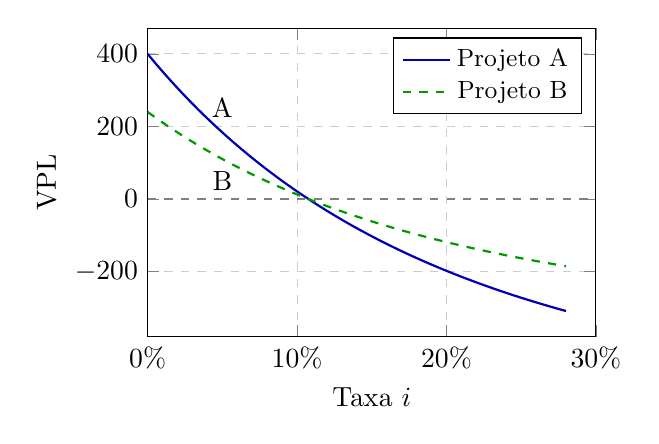
\begin{tikzpicture}
\begin{axis}[
  width=0.6\textwidth, height=5.5cm,
  xlabel={Taxa $i$}, ylabel={VPL},
  xmin=0, xmax=0.3,
  grid=major, grid style={dashed,gray!40},
  xticklabel={\pgfmathparse{\tick*100}\pgfmathprintnumber{\pgfmathresult}\%},
  legend pos=north east, legend style={font=\small},
]
  \addplot[thick, color=blue!70!black, domain=0:0.28, samples=50]
    {1000/(1+x)^5 - 600};
  \addplot[thick, color=green!60!black, dashed, domain=0:0.28, samples=50]
    {600/(1+x)^5 - 360};
  \addplot[dashed, gray] coordinates {(0,0)(0.3,0)};
  \node at (axis cs:0.05,250) {A};
  \node at (axis cs:0.05,50) {B};
  \legend{Projeto A, Projeto B}
\end{axis}
\end{tikzpicture}
\end{center}

Pela TIR, poderíamos escolher B (maior taxa); pelo VPL a taxas baixas, A tem VPL maior.
\textbf{O VPL prevalece}: maximiza a riqueza absoluta do investidor.

\subsection{Projetos com ciclos de vida diferentes}

Quando os projetos têm horizontes distintos, o método da TIR é superior para comparar
a taxa de retorno por período. O VPL de projetos maiores \emph{sempre} será maior --
o que não reflete eficiência.

% ─────────────────────────────────────────────────────────────────────────────
\section{TIR Modificada (TIRM)}

A \textbf{premissa implícita da TIR} é que as receitas intermediárias são reinvestidas
à \emph{própria TIR}. Isso é irreal em muitos contextos.

\begin{definicao}
A \textbf{TIRM} reinveste as receitas à taxa de mercado $i$ e compara com o valor
presente dos investimentos:
\[
  P(1+\TIR M)^n = R\left[\frac{(1+i)^n-1}{i}\right].
\]
\end{definicao}

\begin{resultado}
\[
  P\,(1+\TIRM)^n = \sum_{t=1}^n R_t(1+i)^{n-t}
  \quad\Rightarrow\quad
  \TIRM = \left(\frac{\text{Valor acumulado das receitas}}{P}\right)^{1/n} - 1.
\]
\end{resultado}

\begin{exemplo}{Comparação TIR vs.\ TIRM (Exemplo 6.4)}
Projeto: $P = 50{.}000$, $R = 7{.}500/\text{ano}$, $n = 10$, $i_{\text{mercado}} = 6\%$ a.a.

\medskip
\textbf{TIR:}
\[
  50{.}000 = 7{.}500\left[\frac{(1+r)^{10}-1}{r}\right]\frac{1}{(1+r)^{10}}
  \quad\Rightarrow\quad \TIR \approx 8{,}15\%.
\]

\textbf{VPL} ($i = 6\%$):
\[
  \VPL = 7{.}500\left[\frac{(1{,}06)^{10}-1}{0{,}06}\right]\frac{1}{(1{,}06)^{10}} - 50{.}000
       \approx \textbf{R\$\,5.200{,}65.}
\]
\end{exemplo}

% ─────────────────────────────────────────────────────────────────────────────
\section{Índice de Sharpe e Risco}

Para comparar ativos com diferentes perfis de risco, define-se o \textbf{retorno histórico}:
\[
  r_t = \frac{P_t - P_{t-1}}{P_{t-1}},
  \qquad
  \bar{r} = \frac{1}{n}\sum_{t=1}^n r_t.
\]
A \textbf{volatilidade} (desvio-padrão dos retornos):
\[
  \sigma = \sqrt{\frac{\sum_{t=1}^n (r_t - \bar{r})^2}{n-1}}.
\]

\begin{definicao}
O \textbf{Índice de Sharpe} mede o excesso de retorno por unidade de risco:
\[
  S_i = \frac{r_i - r_f}{\sigma_i},
\]
onde $r_f$ é a taxa livre de risco. Quanto maior $S_i$, melhor o ativo em termos de risco--retorno.
\end{definicao}

\begin{moderno}[title={Análise de projeto de energia solar (2025)}]
Uma empresa estuda instalar painéis solares com:
\begin{itemize}[leftmargin=1.8em, nosep]
  \item Investimento inicial: R\$\,120.000.
  \item Economia anual em energia (fluxo de caixa): R\$\,20.000/ano por 10 anos.
  \item Taxa de desconto (WACC): $8\%$ a.a.
\end{itemize}
\[
  \VPL = 20{.}000\left[\frac{(1{,}08)^{10}-1}{0{,}08}\right]\frac{1}{(1{,}08)^{10}} - 120{.}000
       \approx \textbf{R\$\,14.205.}
\]
Como VPL $> 0$, o projeto cria valor. A TIR implícita $\approx 10{,}56\%$ a.a., superior ao WACC de $8\%$.
Com créditos de carbono adicionando R\$\,2.000/ano, o VPL sobe para $\approx$ R\$\,27.600.
\end{moderno}
